\documentclass{article}[12pt, letter]
\usepackage[left=1in,top=1in,bottom=1in,right=1in]{geometry}
\usepackage{graphicx}
\usepackage{amsmath}
\usepackage{amssymb}

\title{Lattice Theory of Information}
\author{C.E. Shannon}
\date{}

\begin{document}


\maketitle

\begin{abstract}
	The word ``information" has been given many different meanings by various writers in the general field of information theory. It is likely that at
	least a number of these will prove sufficiently useful in certain applications to deserve further study and permanent recognition. It is hardly to be
	expected that a single concept of information would satisfactorily account for the numerous possible applications of this general field. The present note outlines a new approach to information theory which is aimed specifically at the analysis of certain communication problems in which there exist a number of information sources simultaneously in operation. A typical example is that 	of a simple communication channel with a path from the receiving point to the transmitting point. The problem is to make use of the feedback information for improving forward transmission, and to determine the forward channel capacity when the best possible use is made of this feedback information. Another more general problem is that of a communication system consisting of a large number of transmitting and receiving points with some type of interconnecting network between the various points. The problem here is to formulate the best systems design whereby, in some sense, the best overall use of the available facilities is made. While the analysis sketched here has not yet proceeded to the point of a complete solution of these problems, partial answers have been found and it is believed that a complete solution may be possible.
\end{abstract}

\section{The Nature of Information}

In communication theory we consider information to be produced by a suitable stochastic process. We consider here only the discrete case; the
successive symbols of the message are chosen from a finite ``alphabet" and it is assumed for mathematical simplicity that the stochastic process producing the message has only a finite number of possible internal states. The message itself is then a discrete time series which is one sample from the ensemble of possible messages that might have been produced by the information source. The entropy $H(x)$ of such a source is a measure of the amount of information produced by the source per letter of message. However, $H(x)$ can hardly be said to represent the actual information. Thus, two entirely different sources might produce information at the same rate (same $H$) but certainly they are not producing the same information.

To define a concept of actual information, consider the following situation. Suppose a source is producing, say, English text. This may be translated or encoded into many other forms (e.g. Morse code) in such a way that it is possible to decode and recover the original. For most purposes of communication, any of these forms is equally good and may be considered to contain the same information. Given any particular encoded form, any of the others may be obtained, (although of course it may require an involved computation to do so). Thus we are led to define the actual information of a stochastic process as that which is common to all stochastic processes which may be obtained from the original by reversible encoding operations. It is desirable from a practical standpoint and mathematically convenient to limit the kind of all allowed encoding operations in certain ways. In particular, it is desirable to require that the encoding operations be done by a transducer with a finite number of possible internal states. This finite memory condition prevents paradoxical situations in which information goes into a transducer more rapidly on the average than it comes out at the output.

Each encoded version of the original process may be called a \textit{translation} of the original language. These translations may be viewed as different ways of describing the same information in about the same way that a vector may be described by its components in various coordinate systems. The information itself may be regarded as the equivalence class of all translations or ways of describing the same information.

\section{The Metric, Topology and Convergent Sequences}

With this definition of information, it is possible to set up a metric satisfying the usual requirements. The metric $\rho(x,y)$ measures the distance between two information elements $x$ and $y$, and is given in terms of conditional entropies.%
% \endnote{Now, $H(x \vert y)$ is more common notation for Shannon's $H_y(x)$.}
We define
\[
\rho(x, y) = H_x(y) + H_y(x) = 2 H(x,y) - H(x) - H(y).
\]
The symmetry property $\rho(x,y) = \rho(y,x)$ is obvious from the definition. If $\rho(x,y) = 0$, both $H_x(y)$ and $H_y(x)$ must be zero (since both are necessarily non-negative), and this requires that the $x$ sequence be calculable with probability $1$ from the $y$ sequence and vice versa. The triangle law for the metric
\[
\rho(x,y)  + \rho(y,z) \geq \rho(x,z)
\]
is readily shown by expanding these terms into various entropies and making use of known inequalities for entropies. It may be noted that $\rho(x,y)$ is independent of the particular translations of $x$ and $y$ used in its calculation. This is due to the fact that $H_x(y)$ and $H_y(x)$ are invariant under finite state encoding operations applied to $x$ and $y$.

The existence of a natural metric enables us to define a topology for a set of information elements and in particular the notion of sequences of such elements which approach a limit. A set of information elements $x_1, x_2, \dots, x_n, \dots$ will be said to be Cauchy convergent if 
\[
\lim_{m \to \infty} \rho(x_m,x_n) = 0.
\]
The information of these sequences as new elements (analogous to irrational numbers) completes the space in a satisfactory way and enables one to simplify the statement of various results.

\section{The Information Lattices}

A relation of inclusion $x \geqslant y$, between two information elements $x$ and $y$ can be defined by
\[
x \geqslant y \quad \textrm{if and only if} \quad H_x(y) = 0.
\]
This essentially requires that $y$ be obtained by a suitable finite state operation (or limit of such operations) on $x$. If $x \geqslant y$ we call $y$ an \textit{abstraction} of $x$. If $x \geqslant y$, $y \geqslant z$, then $x \geqslant z$. If $x \geqslant y$, then $H(x) \geq H(y)$.
Also $x > y$ means $x \geqslant y$, $x \neq y$. The information element, one of whose translations is the process which always produces the same symbol, is the $0$ element, and $x \geqslant 0$ for any $x$.

The \textit{sum} of two information elements, $z = x + y$, is the process one of whose translations consists of the ordered pairs $(x_n, y_n)$ where $x_n$ is the $n$th symbol produced by the $x$ sequence and similarly for $y_n$. We have $z \geqslant x$, $z \geqslant y$ and there is no $w < z$ with these properties; $z$ is the least upper bound of $x$ and $y$. The element $z$ represents the total information of both $x$ and $y$.

The \textit{product} $z = x y$ is defined as the largest $z$ such that $z \leqslant x$, $z \leqslant y$; that is, there is no $w > z$ which is any abstraction of both $x$ and $y$. The product is unique. Here $z$ is the common information of $x$ and $y$.

With these definitions a set of information elements with all their sums and products forms a metric lattice. The lattices obtained in this way are not, in general, distributive, or even modular.
However they can be made to be relatively complemented by the addition of suitable elements. For $x \leqslant y$ it is possible to construct an element $z$ with
\begin{align*}
	z + x = y \\
	z x = 0.
\end{align*}
The element $z$ is not, in general, unique.

The lattices obtained from a finite set of information sources are of a rather general type; they are at least as general as the class of finite partition lattices. With any finite partition lattice it is possible to construct an information lattice which is abstractly isomorphic by a simple procedure.

\noindent Some example of simple information lattices are shown in Figs.~\ref{fig:1} and \ref{fig:2}.

In Fig.~\ref{fig:1}, there are three independent sources. The product of any two of these elements is zero, and the conventional lattice diagram is that shown at the right. In Fig.~\ref{fig:2}, there are two independent sources of binary digits, $x$ and $y$. The sequence $z6$ is the sum modulo $2$ of corresponding symbols from $x$ and $y$. In this case again the product of any two of $x$, $y$ and $z$ is zero, but the sum of any two represents the total information in the system. In this case the lattice is non-distributive, since $z y + z x = 0 + 0 = 0$, while $z (x+y) = z \neq 0$.

\begin{figure}
	\begin{center}
		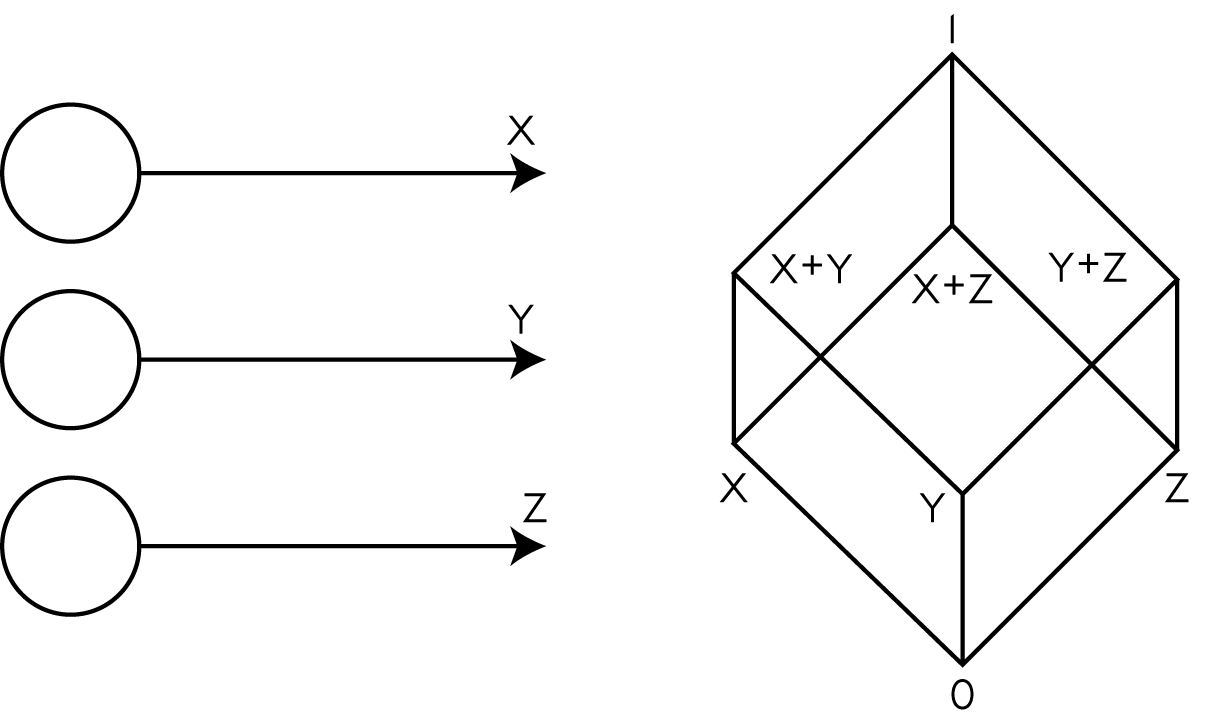
\includegraphics[width=0.5\textwidth]{figs/fig1.png}
		\end{center}
	\caption{}\label{fig:1}
\end{figure}

\begin{figure}
	\begin{center}
		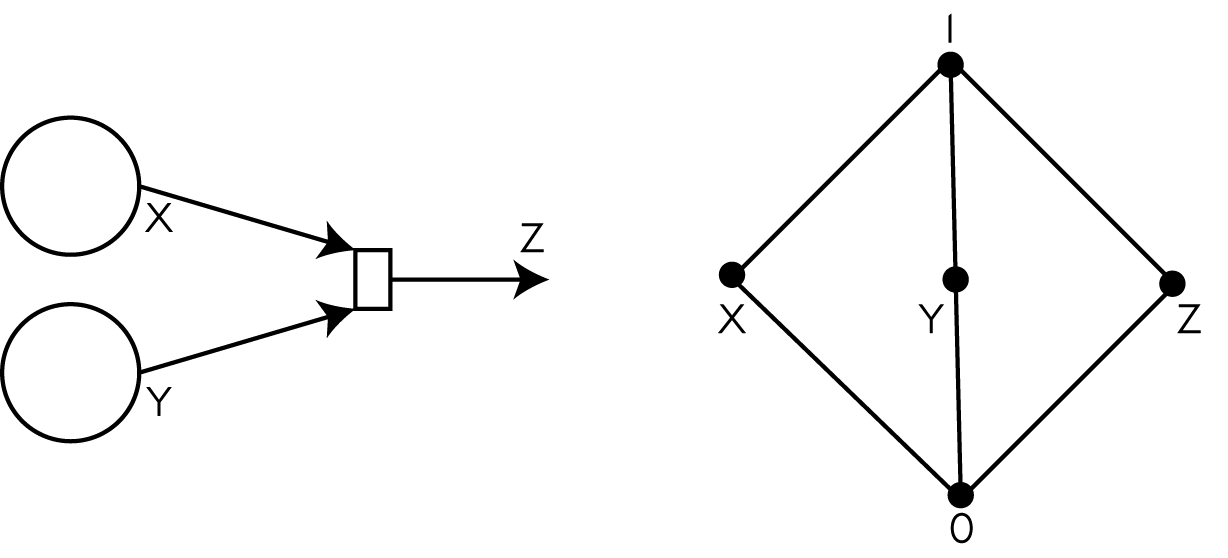
\includegraphics[width=0.5\textwidth]{figs/fig2.png}
	\end{center}
	\caption{}\label{fig:2}
\end{figure}
	


\section{The Delay Free Group $G_1$}

The definition of equality for information based on the group $G$ of all reversible encoding operations allows $x = y$ when $y$ is, for example, a delayed version of $x$; $y_n = x_{n+a}$. In some situations, when one must act on information at a certain time, a delay is not permissible. In such a case we may consider the more restricted group $G_1$ of \textit{instantaneously reversible} translations. One may define inclusion, sum, product, etc., in an analogous way, and this also leads to a lattice but of much greater complexity and with many different invariants.


\end{document}